% Tik output from JumanG
\documentclass[class=minimal,border=0pt]{article}
\usepackage{tikz}
\pagestyle{empty}
\usepackage{verbatim}
\begin{document}
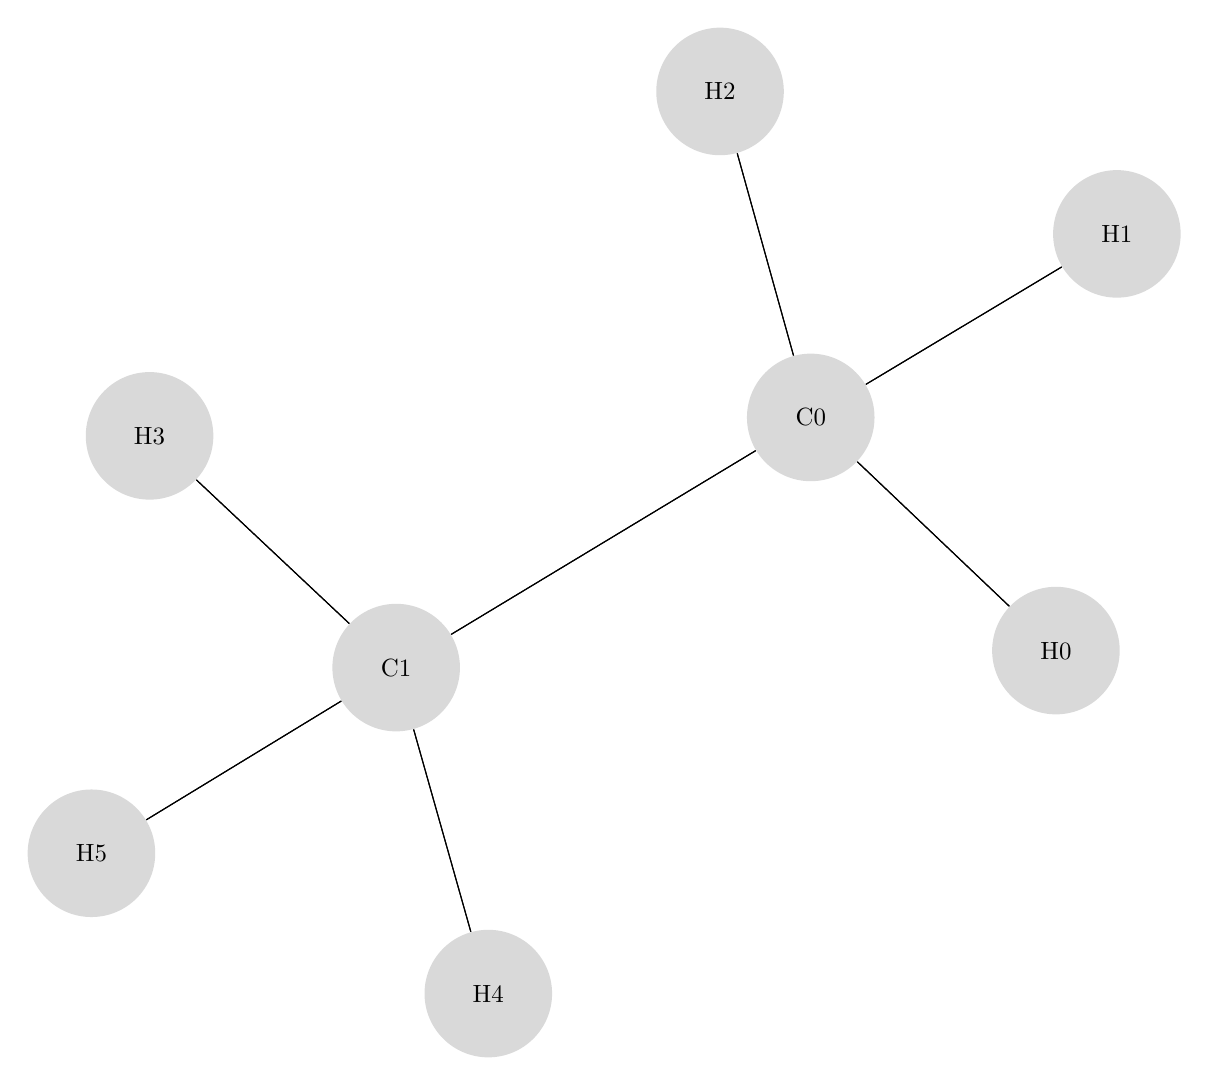
\begin{tikzpicture}[scale=0.90, transform shape]
	\tikzstyle{every node} = [circle, fill=gray!30, minimum size = 1.8cm]
	\node (H4) at (0.16, -4.08) {H4};
	\node (H5) at (-5.44, -2.10) {H5};
	\node (H2) at (3.43, 8.65) {H2};
	\node (H3) at (-4.62, 3.79) {H3};
	\node (H0) at (8.17, 0.76) {H0};
	\node (H1) at (9.03, 6.64) {H1};
	\node (C1) at (-1.14, 0.52) {C1};
	\node (C0) at (4.71, 4.05) {C0};
	\draw [-] (H4)--(C1);
	\draw [-] (H5)--(C1);
	\draw [-] (H2)--(C0);
	\draw [-] (H3)--(C1);
	\draw [-] (H0)--(C0);
	\draw [-] (H1)--(C0);
	\draw [-] (C1)--(C0);
	\draw [-] (C1)--(H3);
	\draw [-] (C1)--(H4);
	\draw [-] (C1)--(H5);
	\draw [-] (C0)--(H0);
	\draw [-] (C0)--(H1);
	\draw [-] (C0)--(H2);
	\draw [-] (C0)--(C1);
\end{tikzpicture}
\end{document}
